\documentclass{report}

\usepackage{graphicx}

\usepackage{pdfpages} 

\usepackage{amsmath}
\usepackage{listings}
\usepackage{color} %red, green, blue, yellow, cyan, magenta, black, white
\definecolor{mygreen}{RGB}{28,172,0} % color values Red, Green, Blue
\definecolor{mylilas}{RGB}{170,55,241}


\title{\textbf{Computational Mathematics - Assignment 2}\\Owen Burke, 15316452}
\begin{document}

    \lstset{language=Matlab,%
    %basicstyle=\color{red},
    breaklines=true,%
    morekeywords={matlab2tikz},
    keywordstyle=\color{blue},%
    morekeywords=[2]{1}, keywordstyle=[2]{\color{black}},
    identifierstyle=\color{black},%
    stringstyle=\color{mylilas},
    commentstyle=\color{mygreen},%
    showstringspaces=false,%without this there will be a symbol in the places where there is a space
    numbers=left,%
    numberstyle={\tiny \color{black}},% size of the numbers
    numbersep=9pt, % this defines how far the numbers are from the text
    emph=[1]{for,end,break},emphstyle=[1]\color{red}, %some words to emphasise
    %emph=[2]{word1,word2}, emphstyle=[2]{style},    
}







    \maketitle
    \section*{\hfil Question 4.23 \hfil}
    Write a user-defined MATLAB function that decomposes an n x n matrix [A] into a lower triangular matrix [L] and an upper triangular matrix [U] (such that [A] = [L][U]) using the 
    Gauss elimination method (without pivoting). For the function name and arguments, use [L,U] = LUdecompGauss(A), where the input argument A is the matrix to be decomposed and the output 
    arguments L and U are the cor­responding upper and lower triangular matrices. Use LUdecompGauss to determine the LU decomposi­tion of the following matrix: 
    
		\subsection*{$\begin{bmatrix}
            4 & -1 & 3 & 2\\
            -8 & 0 & -3 & -3.5\\
            2 & -3.5 & 10 & 3.75\\
            -8 & -4 & 1 & -0.5\\
        \end{bmatrix}$}
                  
        \lstinputlisting{LUdecompGauss.m}

        \begin{figure}[h!]
            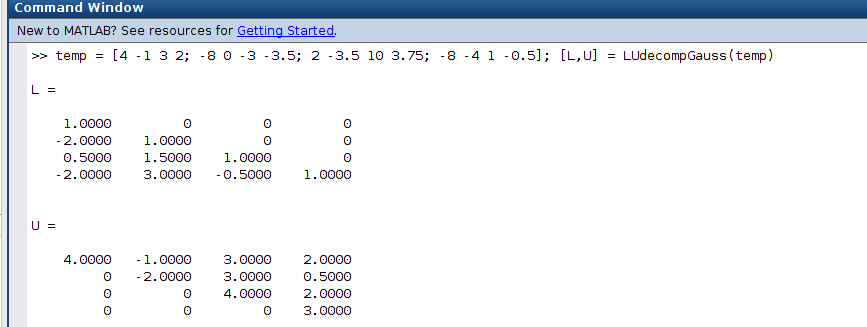
\includegraphics[width=\linewidth]{LUdecompPic.png}
            \caption{LUdecompGauss with matrix above}
            \label{fig:LUdecompPic}
        \end{figure}

    
    \section*{\hfil Question 5.17 \hfil}
    A football conference has six teams. The outcome of the games is recorded in a binary fashion. For example, if team 1 defeats teams 5 and 6, then the equation x\textsubscript{1} = 
    x\textsubscript{5} + x\textsubscript{6} is written to indicate these results. At the end of the season, the wins and loses are tabulated in this fashion to produce the following 
    ranking matrix: 
        
        \subsection*{$\begin{bmatrix}
            x\textsubscript{1}\\
            x\textsubscript{2}\\
            x\textsubscript{3}\\
            x\textsubscript{4}\\
            x\textsubscript{5}\\
            x\textsubscript{6}\\
        \end{bmatrix}$ = $\begin{bmatrix}
                0 & 0 & 0 & 1 & 0 & 0\\
                1 & 0 & 1 & 0 & 1 & 1\\
                0 & 1 & 0 & 0 & 1 & 0\\
                1 & 1 & 0 & 0 & 1 & 0\\
                1 & 1 & 1 & 0 & 0 & 1\\
                1 & 0 & 0 & 0 & 1 & 0\\
            \end{bmatrix}$ $\begin{bmatrix}
                x\textsubscript{1}\\
                x\textsubscript{2}\\
                x\textsubscript{3}\\
                x\textsubscript{4}\\
                x\textsubscript{5}\\
                x\textsubscript{6}\\
            \end{bmatrix}$}
        
    (a) Find the eigenvalues and the corresponding eigenvectors of [A], using MATLAB's built-in function \textit{eig}.\\\\

        \lstinputlisting{eigen_a.m}

        \begin{figure}[h!]
            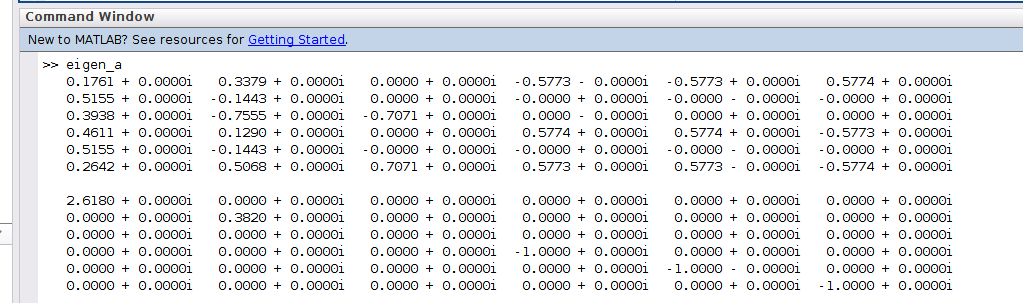
\includegraphics[width=\linewidth]{eigenVals_and_eigenVecs.png}
            \caption{eigenvalues and the corresponding eigenvectors of [A]}
            \label{fig:eigenVals_and_eigenVecs}
        \end{figure}

        \textbf{Eigenvalues and corresponding eigenvectors: *from the matlab execution of \textit{eig} as seen above} \\\\
        $\lambda$ = 2.6180, {$\begin{bmatrix}
                                0.1761 \\
                                0.5155 \\
                                0.3938 \\
                                0.4611 \\
                                0.5155 \\
                                0.2642 \\
                            \end{bmatrix}$}\\\\

        $\lambda$ = 0.3820, {$\begin{bmatrix}
                                0.3379 \\
                                -0.1443 \\
                                -0.7555 \\
                                0.1290 \\
                                -0.1443 \\
                                0.5068 \\
                            \end{bmatrix}$}\\\\

        $\lambda$ = 0.0000, {$\begin{bmatrix}
                                0.0000 \\
                                0.0000 \\
                                -0.7071 \\
                                0.0000 \\
                                -0.0000 \\
                                0.7071 \\
                            \end{bmatrix}$}\\\\

        $\lambda$ = -1.0000, {$\begin{bmatrix}
                                -0.5773 \\
                                -0.0000 \\
                                0.0000 \\
                                0.5774 \\
                                -0.0000 \\
                                0.5773 \\
                            \end{bmatrix}$}\\\\

        $\lambda$ = -1.0000, {$\begin{bmatrix}
                                -0.5773 \\
                                -0.0000 \\
                                0.0000 \\
                                0.5774 \\
                                -0.0000 \\
                                0.5773 \\
                            \end{bmatrix}$}\\\\

        $\lambda$ = -1.0000, {$\begin{bmatrix}
                                0.5774 \\
                                -0.0000 \\
                                0.0000 \\
                                -0.5773 \\
                                -0.0000 \\
                                -0.5774 \\
                            \end{bmatrix}$}\\\\
                            

    (b) Find the eigenvector from part (a) whose entries are all real and of the same sign (it does not matter if they are all negative or all positive), and rank the teams from best 
        (i.e., with most win) to worst (i.e., with fewest wins) based on the indices of the teams corresponding to the largest to the smallest entries in that eigenvector. \\

        From part a), we can see that the eigenvector whose entries are all real and of the same sign is :\\
        {$\begin{bmatrix}
            0.1761 \\
            0.5155 \\
            0.3938 \\
            0.4611 \\
            0.5155 \\
            0.2642 \\
        \end{bmatrix}$}\\\\
        Therefore, we can rank the teams from best to worst corresponding to the largest (0.5155) to the smallest (0.1761) entries in the eigenvector. Giving us :\\
        \textbf{Best (joint)} : x\textsubscript{2}, x\textsubscript{5}\\
        \textbf{2\textsuperscript{nd} best} : x\textsubscript{4}\\
        \textbf{3\textsuperscript{rd} best} : x\textsubscript{3}\\
        \textbf{4\textsuperscript{th} best} : x\textsubscript{6}\\
        \textbf{Worst} : x\textsubscript{1}\\


    
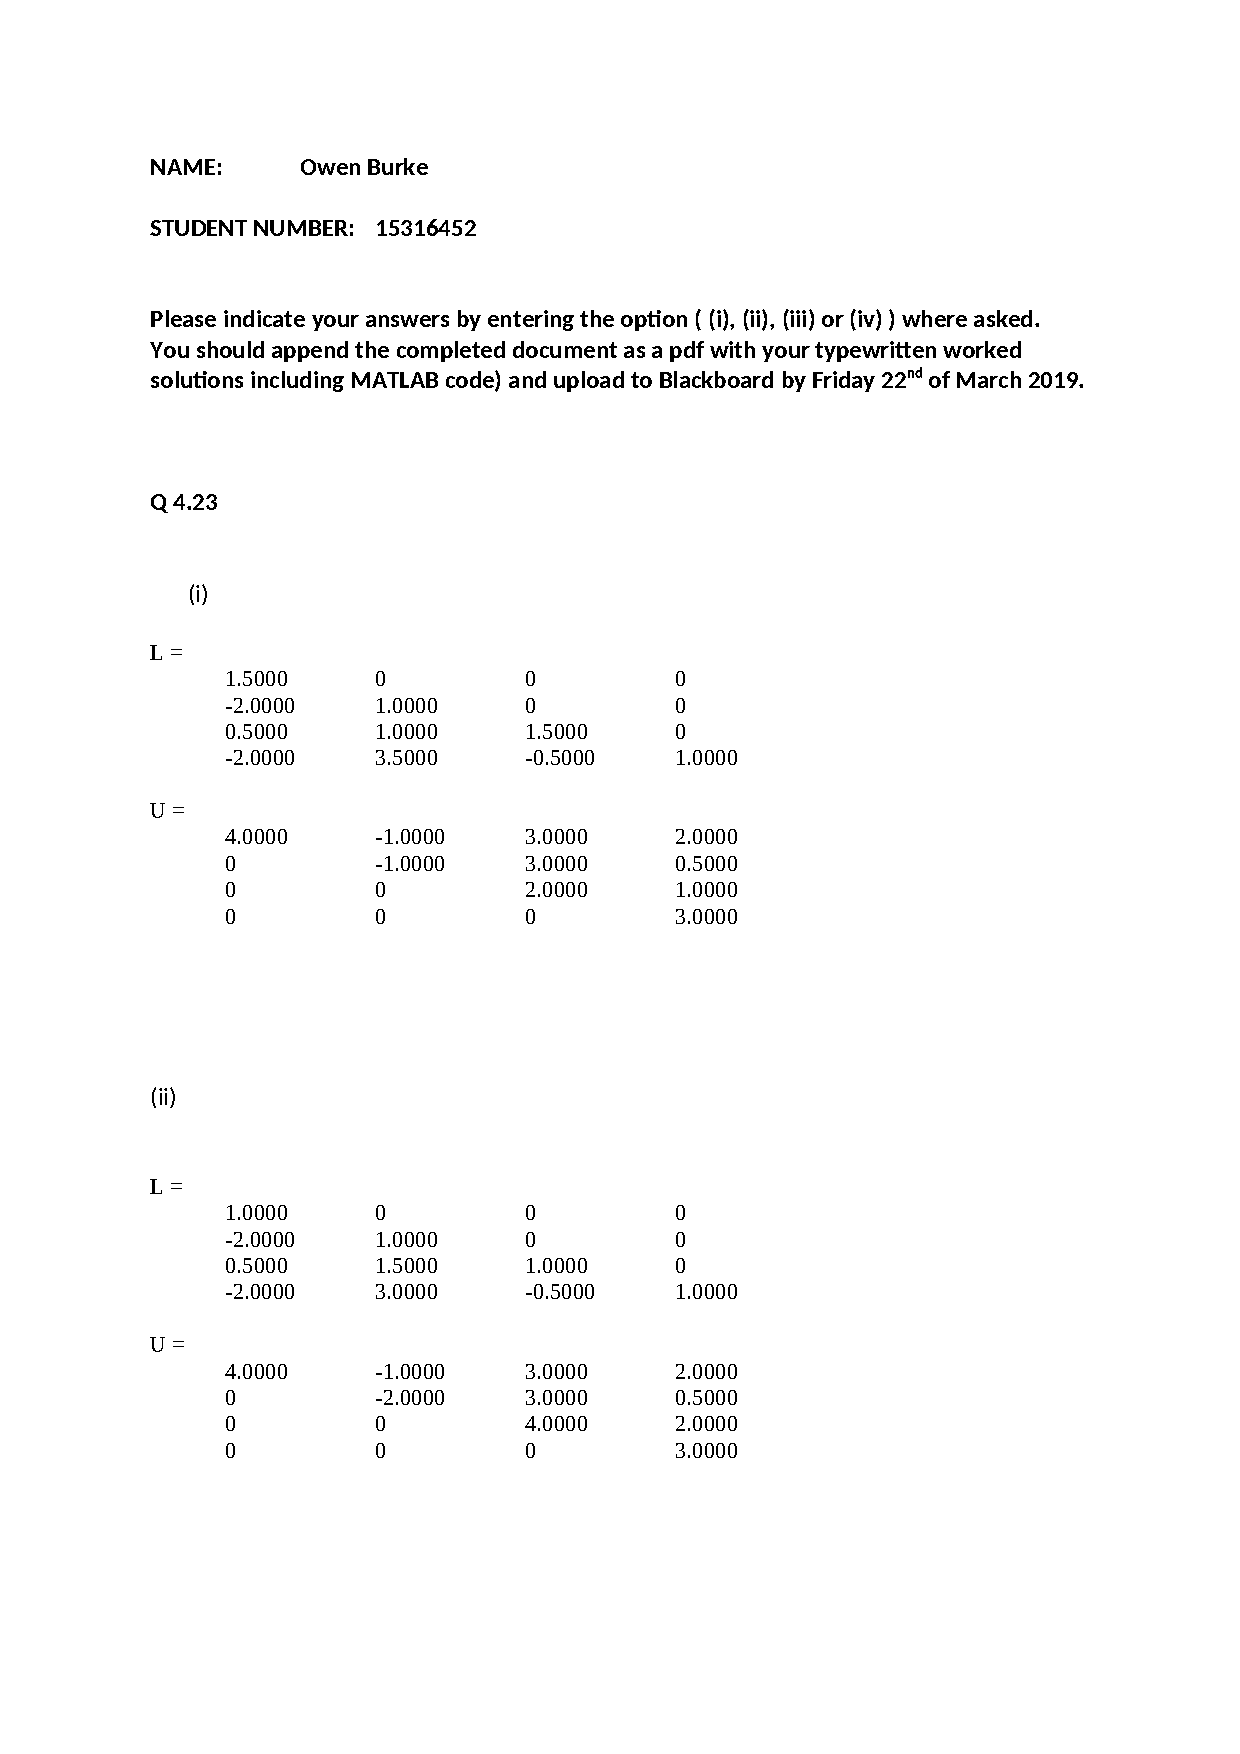
\includepdf[page=-]{CS3081_Assignment_2_Multichoice.pdf}

\end{document}